\scanpage{63}
\figure{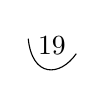
\begin{tikzpicture}\draw (-.30,.14) .. controls (-.25,-.35) and (.10,-.35) .. (.31,-.05);\node at (0,.05) {\mspage{19}};\end{tikzpicture}}
des diagrammes 17, donne une $\unsure{\underline{\mathrm{Lim}}|\underset{\longrightarrow}{\mathrm{Lim}}}$ qui se représente de $=$ comme espace somme, a peu de chances d'être homéo. à $X$ (p. ex. si $X$ conn\ldots) !

Les $\unsure{V_{j,k}^j|V_{i,k}^j}$ sont des germes de sous-espaces de $X$, leurs \unsure{seuls|seules} \deleted{\unsure{relations d'}} \inserted{morphismes} canoniques entre eux sont les morphismes d'inclusions — à quelle condition donc a-t-on
\[
(18)\qquad V_{i,k}^j\subset V_{i',k'}^{j'}
\]
pour
\[
(19)\qquad i\leq j\leq k,\qquad i'\leq j'\leq k'
\]
donnés ? Qu'en est-il pour les espaces élémentaires
\[
X_i^*,\quad V_{i,j}^*,\quad V_{i,j}\qquad(j\text{ successeur de }i)\ ?
\]
Je vais supposer pour simplifier les $X_i^*\ne\varnothing$.
\inserted{(\unsure{alors} $X_i\subset X_j\Longrightarrow i\leq j$ — car sinon on aurait $X_i^*=\varnothing$ justement\ldots)}
Il n'y a donc pas de relations d'inclusions entre les $X_i^*$ pour des indices distincts, \deleted{\unsure{si pour}} \inserted{Si} $V_{i,j}\subset V_{i',j'}$, passant aux ``pts'' \inserted{de $X$''} de ces germes d'espaces, il faut avoir $X_i^*\subset X_{i'}^*$ d'où $i=i'$, donc si on suppose que le germe d'un $X_j$ ($j$ successeur de $i$) le long de $X_i^*$ détermine déjà $j$ (ce qui est bien vraisemblable), on devra avoir aussi $j=j'$. De $=$, on voit que si $V_{ij}^*\subset V_{i',j'}^*$, leurs ens de pts d'adhérence, \deleted{\unsure{situés sur|à savoir} $\overline{X_i^*}$ et $\overline{X_{i'}^*}$}, compris entre $\overline{X_i^*}$ et $X_i$ \inserted{\unsure{resp.|pour} $\overline{X_{i'}^*}$ et $X_{i'}$}, sont en relation d'inclusion,
\mspage{62}
